% !TEX TS-program = lualatex
% -------------------------------------------------------------------------------
% This document provides a template for a presentation in the style of the 
% University of Waterloo, Waterloo, Canada.
%
% The LaTeX template is released under the GNU Lesser General Public License. 
% The following applies:
% The LaTeX template is free software: you can redistribute it and/or modify
% it under the terms of the GNU Lesser General Public License as published by
% the Free Software Foundation, either version 3 of the License, or
% (at your option) any later version.
%
% The LaTeX template is distributed in the hope that it will be useful,
% but WITHOUT ANY WARRANTY; without even the implied warranty of
% MERCHANTABILITY or FITNESS FOR A PARTICULAR PURPOSE. See the
% GNU Lesser General Public License for more details.
%
% You should have received a copy of the GNU Lesser General Public License
% along with the JAMS Python package (cf. gpl.txt and lgpl.txt).
% If not, see <http://www.gnu.org/licenses/>.
%
% Copyright 2016-2016 Juliane Mai
% -------------------------------------------------------------------------------

\documentclass{beamer}                  % use beamer class
%%%%%%%%%%%%%%%%%%%%%%%%%%%%%%%%%%%%%%%%%%%%%%%%%%%%%%%%%%%
%% Beamer class source. (original from:  Sascha Frank)   %%
%%           Author:    Christoph L. Schneider           %%
%%             Date:    Apr 2008                         %%
%%          Compile:    pdflatex                         %%
%%%%%%%%%%%%%%%%%%%%%%%%%%%%%%%%%%%%%%%%%%%%%%%%%%%%%%%%%%%
%% use style file 'Leipzig' for colors, fonts and layout %%
%% leave those options empty, you do NOT wish            %%
%%                                                       %%
%% OPTIONS                                               %%
%% (a) turn on page numbers at the bottom line: numbers  %%
%% (b) turn on flowchart bar at the top line: flowchart  %%
%% (c) turn on navigation bar at the bottom line: nav    %%
%%                                                       %%
\usetheme[numbers]{WaterlooYellow}             %%
%%                                                       %%
%% e.g. set all options                                  %%
%% \usetheme[numbers,flowchart,nav]{Leipzig}             %%
%% or only numbers                                       %%
%% \usetheme[numbers]{Leipzig}                           %%
%%%%%%%%%%%%%%%%%%%%%%%%%%%%%%%%%%%%%%%%%%%%%%%%%%%%%%%%%%%

% ----------------------------------------------
% import some additional packages
% ----------------------------------------------
\usepackage{fontspec}
\usepackage{fontawesome}  
\usepackage{graphicx}  % Required for including images
\usepackage{caption}              % to include figures
\usepackage{tikz}                       % to draw some simple stuff
\usetikzlibrary{patterns}               % to use paterns for TikZ drawings
\usetikzlibrary{shapes,arrows}          % to use arrows and shapes in TikZ drawings
%\usepackage[german,ngerman]{babel}      % special GERMAN hyphenation, quotes, characters, 
%%                                       % dates and labeling like 'Abb.', 'Tabelle', etc.
%\usepackage[utf8]{inputenc}             % translation of GERMAN umlauts in editor to document
\usepackage[english]{babel}             % ENGLISH hyphenation, quotes, dates and labeling like 'Figures', 'Table', etc.
\usepackage{amsmath}                    % mathematical typesetting
\usepackage{amssymb}                    % special symbols for math mode
\usepackage{wasysym}                    % some more special characters
\usepackage[absolute,overlay]{textpos}  % to position textblocks at arbitary places - must be after color

\usepackage[noend]{algpseudocode}
\usepackage{algorithm}

\usepackage{tabularx}
\usepackage{booktabs}
\newcolumntype{Y}{>{\centering\arraybackslash}X}
\newcolumntype{R}{>{\raggedleft\arraybackslash}X}  %% right aligned
\usepackage{ragged2e}

% ----------------------------------------------
% define UFZ/UW standard colors
% ----------------------------------------------
\definecolor{ufzdarkblue}{RGB}{0,62,110}
\definecolor{ufzblue}{RGB}{0,88,156}
\definecolor{ufzlightblue}{RGB}{0,162,224}
\definecolor{ufzred}{RGB}{212,45,18}
\definecolor{ufzorange}{RGB}{207,104,0}
\definecolor{ufzyellow}{RGB}{230,175,17}
\definecolor{ufzdarkgreen}{RGB}{20,77,40}
\definecolor{ufzgreen}{RGB}{169,181,9}
\definecolor{ufzgray1}{RGB}{81,81,81}
\definecolor{ufzgray2}{RGB}{156,156,156}
\definecolor{ufzgray3}{RGB}{185,185,185}
\definecolor{ufzblack}{RGB}{0,0,0}
\definecolor{ufzwhite}{RGB}{255,255,255}
\definecolor{uwred}{RGB}{183,18,52}
\definecolor{uwyellow1}{RGB}{254,250,170}  % 1st color in stripe
\definecolor{uwyellow2}{RGB}{252,234,47}   % 2nd color in stripe
\definecolor{uwyellow3}{RGB}{251,213,79}   % 3rd color in stripe
\definecolor{uwyellow4}{RGB}{228,180,42}   % 4th color in stripe (mostly used)
\definecolor{uwyellow5}{RGB}{251,223,75} 
\definecolor{uwyellow}{RGB}{234,199,81}    % yellow text

% ----------------------------------------------
% width and height units for positioning textblocks
% ----------------------------------------------
\setlength{\TPHorizModule}{1cm} 
\setlength{\TPVertModule}{1cm}

% ----------------------------------------------
% spaces in lists
% ----------------------------------------------
\addtolength{\partopsep}{-5pt} % lists: extra space added to \topsep when environment starts a new paragraph.
\addtolength{\topsep}{-3pt}    % lists: space between first item and preceding paragraph.
\addtolength{\itemsep}{-5pt}   % lists: space between successive items.
\addtolength{\floatsep}{-20pt} % space left between floats, i.e. tables and figures

% ----------------------------------------------
% define own commands:
% (a) \UFZ{xxx}        to change textcolor of xxx to blue
% (b) \rmlogo          to remove logo of UFZ on a slide
% (c) \UWtitle{xxx}   to set caption of a slide centered and in blue color
% (d) \fillframe       to fill a slide with vertical space such that text do not get centered
% ----------------------------------------------
%
% (a) Blue text
\newcommand{\UFZ}[1]{\textcolor{ufzblue}{#1}}
\newcommand{\UW}[1]{\textbf{\textcolor{black}{#1}}}
%\newcommand{\UW}[1]{\textbf{\textcolor{uwyellow4}{#1}}}
%
% (b) Overlay UFZ logo with white box
\newcommand{\rmlogo}{
	\begin{textblock}{2.7}(9.55,8.65)
		{\color{white}\rule{2.85cm}{0.7cm}}
	\end{textblock}
}

\newcommand{\rmemblem}{
	% without flowchart
	%	\begin{textblock}{2.7}(9.3,0.0)
	%		{\color{white}\rule{3.6cm}{7.4cm}}
	%	\end{textblock}
	% with flowchart
	\begin{textblock}{2.7}(9.3,0.43)
		{\color{white}\rule{3.6cm}{7.4cm}}
	\end{textblock}
}
%
% (c) Slide title
\newcommand{\UWtitle}[1]{
	\begin{textblock}{12.8}(0.0,0.7)
		\begin{center} 
			\textbf{\UW{\Large{#1}}}
		\end{center}
	\end{textblock}
}

\setbeamerfont{headline}{size=\fontsize{5}{5}\selectfont}
\setbeamercolor{headleft}{fg=ufzdarkgreen, bg=uwyellow1}
\setbeamercolor{headmid}{fg=ufzgray1, bg=uwyellow5}
\setbeamercolor{headright}{fg=ufzblack, bg=uwyellow4}
\setbeamertemplate{headline}
{
 \hbox{%
  \begin{beamercolorbox}[wd=.33\paperwidth,ht=2.6ex,dp=1ex,center]{headleft}%
    \usebeamerfont{headleft}{Guiwen Luo}
  \end{beamercolorbox}%
  \begin{beamercolorbox}[wd=.34\paperwidth,ht=2.6ex,dp=1ex,center]{headmid}%
    \usebeamerfont{headleft}{Abbr. of the Title}
  \end{beamercolorbox}%
  \begin{beamercolorbox}[wd=.33\paperwidth,ht=2.6ex,dp=1ex,center]{headright}%
    \usebeamerfont{headright} \text{Slide  } \insertframenumber/\inserttotalframenumber
  \end{beamercolorbox}}%
  \vskip0pt%
}



% (d) Fill up the rest of slide so that text does not get centered
\newcommand{\fillframe}{\vspace*{10cm}}

%Guiwen_Luo's Self-defined set of shortcut inputs for frequently-used symbols
{
\newcommand{\FF}{\mathbb{F}}
\newcommand{\FFq}{\mathbb{F}_q}
}



 \newcommand{\BL}[1]{\textcolor{blue}{\textbf{#1}}}
 \newcommand{\RE}[1]{\textcolor{red}{\textbf{#1}}}
 \newcommand{\GN}[1]{\textcolor{green}{\textbf{#1}}}

\usebackgroundtemplate{
\includegraphics[width=\paperwidth,height=\paperheight]
	{Figures/uwaterloo_background_white.pdf}}


%%%%%%%%%%%%%%%%%%%%%%%%%%%%%%%%%%%%%%%%%%%%%%%%%%%%%%%%%%%%

\begin{document}
	

\begin{frame}
\vspace*{2cm}
\begin{center}
{\Large \UW{Title of the Presentation}}\\
\vspace*{.3cm}
\UW{Guiwen Luo}\\

\vspace*{0.3cm}
        \small{Department of Electrical and Computer Engineering\\
          University of Waterloo\\
                CANADA\\
                \texttt{guiwen.luo@uwaterloo.ca}}
                \\
        \vspace*{0.3cm}
        \normalsize{insert Date}\\
\vspace*{0.3cm}
% [Stinson66-NADCC, 2022]
\normalsize{Joint work with xxx}\\
\end{center}

\fillframe
\end{frame}


%%%%%%%%%%%%%%%%%

   
\begin{frame}
%    \UWtitle{Problem: MSM over fixed points}
    
    
    \begin{block}{Problem:}
    	Multi-scalar Multiplication (MSM) over fixed points: 
    	\begin{equation}\label{eq_multi_scalar_multiplication}
				S_{n,r} = a_1P_1+a_2P_2+...+a_nP_n,\ 0\le a_i< r, P_i\in E.				
				\end{equation}
    \end{block}
How can we compute it efficiently for large $n: n\ge 2^{10}$?

\end{frame}

\begin{frame}
	\UWtitle{Outline}
%	\vspace*{2.5cm}
	\begin{itemize}
	\item Introduction
	\item Existing methods
	\item Pippenger's bucket method and its variant
	\item Our new construction
	\item Instantiation and experiment over BLS12-381 curve
	\end{itemize}
%	\fillframe
\end{frame}


%%%%%
\begin{frame}


\UWtitle{Motivation}

\begin{itemize}
	\item MSM over fixed points dominates the time consumption in zero-knowledge succinct non-interactive argument of knowledge (zkSNARK) schemes with  pairing-based trusted setup.		
			
			\item 	 Circuit size in Zcash: for single hash, SHA-256, the number of multiplication gates is about 23 thousands; for nested hash, several millions.

\end{itemize}

\vspace{0.25in}

\begin{center}
		\begin{figure}
			\centering
			
\includegraphics[width=0.4\linewidth]{Figures/Zcash_logo}
			\captionsetup{labelformat=empty}
			\caption{\centering \footnotesize credit: \url{https://en.wikipedia.org/wiki/Zcash}}
		\end{figure}
\end{center}
							
\end{frame}

%%%%%%%%%%%%%%%%%%%%

\begin{frame}
\small
    \UWtitle{Existing methods}
%    \vspace*{1.3cm}
    \BL{ Computing $S_{n,r}$:}
        \begin{itemize}
           \item<1-> \RE{Binary method}: \\
           doubling-and-addition, \\
           Knuth's 5 window algorithm \cite{knuth1997art, bos1989addition}.
           \item<2-> \BL{Construction of number systems}: \\
           basic digit sets \cite{matula1982basic, brickell1992fast},\\ 
           multi-base number systems \cite{doche2009double,suppakitpaisarn2012fastest, yu2013joint}.
           
           \item<3-> \BL{Addition chains}:  \\
           PRAC chains \cite{montgomery1992evaluating},\\
           DJB chains \cite{bernstein2006differential},\\
           other multi-dimensional differential addition chains \cite{brown2015multi,rao2015note}.
           
           \item<4-> \RE{Pippenger's bucket method and its variants}.
        \end{itemize}
\end{frame}

\begin{frame}
    \UWtitle{Existing methods (cont.)}
    \vspace*{2.5cm}
    \begin{block}{
 For large $n$ ($n\ge 2^{10}$)}
     
     \vspace{0.2in}
        \begin{itemize}
           \item 
           SOTA: Pippenger's bucket method and its variants.
           \vspace{0.2in}
           
           \item zkSNARK-oriented implementations, Zcash, TurboPLONK, Bellman, gnark, choose Pippenger's bucket method.
        \end{itemize}
        \end{block}
   \fillframe
\end{frame}

\begin{frame}
	\UWtitle{Pippenger's bucket method}
	\vspace*{0.8cm}
	\begin{small}
			\begin{itemize}	
				\item<1-> Example:
				\begin{eqnarray*}
				S_{13,8}=2 P_{1}+3 P_{2}+7 P_{3}+6 P_{4}+5 P_{5}+1 P_{6}+3 P_{7}\\
				+6 P_{8}+2 P_{9}+7 P_{10}+1 P_{11}+4 P_{12}+5 P_{13}.
				\end{eqnarray*}
				
				\item<2-> All points are sorted into 7 buckets according to the scalars $\{1, \cdots, 7\}$:
				\begin{equation*}
				\begin{aligned}
				S_{13,8}=& 1 \cdot\left(P_{6}+P_{11}\right)+2 \cdot\left(P_{1}+P_{9}\right)+3 \cdot\left(P_{2}+P_{7}\right)+4 \cdot\left(P_{12}\right) \\
				&+5 \cdot\left(P_{5}+P_{13}\right)+6 \cdot\left(P_{4}+P_{8}\right)+7 \cdot\left(P_{3}+P_{10}\right) \\
				=:& 1 S_{1}+2 S_{2}+\ldots+7 S_{7}.\\
				\end{aligned}
				\end{equation*}					
				\only<3> {The accumulated sum $\sum_{i=1}^{7}iS_i$ can be computed via
				\begin{equation*}
				\begin{aligned}
				&\ \ \ \ \  S_7 \\
				&+ (S_7+S_6)\\
				&+ (S_7+S_6+S_5)\\
				&\cdots \\
				&+(S_7+S_6+S_5+\cdots +S_1).
				\end{aligned}
				\end{equation*}	}			
				
				\item<4-> $\{S_i\}$: $13 - 7 = 6$ additions,\\
				$\sum_{i = 1}^{7} iS_i$: $2\times 6 = 12$ additions. \\
				In total, 18 additions.	
			\end{itemize}
	\end{small}
	\fillframe
\end{frame}

\begin{frame}
	\UWtitle{Pippenger's bucket method}
	\vspace*{1.5cm}
			\begin{itemize}	
				\item If $r$ is small enough:
				\begin{eqnarray*}
				S_{n,r}= a_1P_1+a_2P_2+\cdots + a_nP_n.
				\end{eqnarray*}
				
				\item All points are sorted into $r-1$ buckets according to the scalars,
				\begin{equation*}
				\begin{aligned}
				S_{n,r}=& 1 S_{1}+2 S_{2}+\ldots+(r-1) S_{r-1}\\
				=& S_{r-1} + (S_{r-1}+S_{r-2})+\cdots +(S_{r-1}+S_{r-2}+\cdots +S_1).
				\end{aligned}
				\end{equation*}
				
				\item $S_i$'s: $n - (r -1)$ additions,\\
				$\sum_{i = 1}^{r-1} iS_i$: $2\times (r-2)$ additions.\\
				In total, $n+r -3$ additions.	
			\end{itemize}
	\fillframe
\end{frame}

\begin{frame}
	\UWtitle{Pippenger's bucket method variant}
	\vspace*{1.5cm}
			\begin{itemize}	
				\item<1-> If $r$ is big (over BLS12-381 curve, $r\approx 2^{255}$), every scalar is decomposed into $q$-ary form,
				\begin{eqnarray*}
				a_i &=& a_{i0} + a_{i1}q +\cdots+ a_{i,h-1}q^{h-1} \\
				S_{n,r}&=& a_1P_1+a_2P_2+\cdots + a_nP_n\\
				&=&\sum _{i=1}^n\sum_{j=0}^{h-1}a_{ij}\cdot (q^{j}P_i), 0 \le a_{ij}< q,\\
				& =: & S_{nh,q}.
				\end{eqnarray*}
				
				\item<2-> Precomputation ($nh$ Points):
				\begin{equation*}
				\{q^{j}P_i\ |\ i= 1,2,...,n,\ j=0,1,2,...,h-1\}. 
				\end{equation*}
				
				\item<2-> Using aforementioned method, all points are sorted into $q-1$ buckets,
				in total, $nh+ q -3$ additions \cite{brickell1995fast}.	
			\end{itemize}
	\fillframe
\end{frame}


\begin{frame}
	\UWtitle{Generalized framework}
	\vspace*{1.0cm} 
	\begin{small}
			\begin{itemize}	
				\item<1-> Let us summary the framework of computing MSM,
				$$ S_{n,r} = S_{hn,q}=\sum_{i=1}^{n}\sum_{j=0}^{h-1} a_{ij}q^j P_i, 0\le a_i\le q $$
				
				\item<1-> If $a_{ij} = m_{ij}b_{ij}$, $m_{ij}\in M$ (multiplier), $b_{ij}\in B$ (bucket),
					\begin{equation*}
					\begin{aligned}
					S_{hn,q}&= \sum_{i=1}^{n}\sum_{j=0}^{h-1}b_{ij}\cdot (m_{ij}q^jP_i).\\
					\end{aligned} 
					\end{equation*}
				\item<2-> Precompute ($nh|M|$ points) \\
				$\{mq^jP_i\ |\ 1\le i\le n,0\le j\le h-1,m\in M\}$,\\
				then it takes $\approx nh +|B|$ additions to compute $S_{n,r}$.
				
				\only<3> {\item Pippenger's bucket method variant,
				$M =\{1\},\ B =\{0,1,2,...,q-1\}$, it takes $\approx nh + q$ additions.}
				\item<4-> Pippenger's bucket method variant 2 (notice that $-P$ can be easily computed given $P$),\\
				$M =\{1,-1\},\ B =\{0,1,2,...,\lceil q/2\rceil\}$, it takes $\approx nh + q/2$ additions.
			\end{itemize}
		\end{small}
	\fillframe
\end{frame}

\begin{frame}
	\UWtitle{ }
%	\vspace*{3cm} 
			\begin{center}	
			   \begin{block}{Goal:}
				Construct $B$, \textit{s.t.} $|B|\approx 0.21q$. Thus $S_{n,r}$ takes $\approx nh + 0.21q$ additions.
				\end{block}
			\end{center}
%	\fillframe
\end{frame}

\begin{frame}
\small
	\UWtitle{New construction}
	\vspace*{0.9cm}

		\begin{itemize}	
			\item<1-> (G.W. Luo, S.H. Fu,  G. Gong) Let $q = 2^c$ be the radix. The multiplier set is 
			$M =\{-3,-2,-1,1,2,3\}$.
			\item<2->  Three auxiliary sets,
			\begin{equation*}
			\begin{aligned}
			B_0 =& \{0\} \cup \{b\ |\ 1\le b \le q/2, s.t.\ \omega_2(b) +\omega_3(b) \equiv 0 \bmod 2 \},\\
			B_2 =& \{0\} \cup \{b\ |\ 1\le b \le r_{h-1}+1, s.t.\ \omega_2(b) +\omega_3(b) \equiv 0 \bmod 2 \},
			\end{aligned}
			\end{equation*}
			where $r_{h-1}=\lfloor r/q^{h-1}\rfloor$. $B_1$ is defined by the following algorithm
				\begin{center}
				\begin{figure}
					\centering
					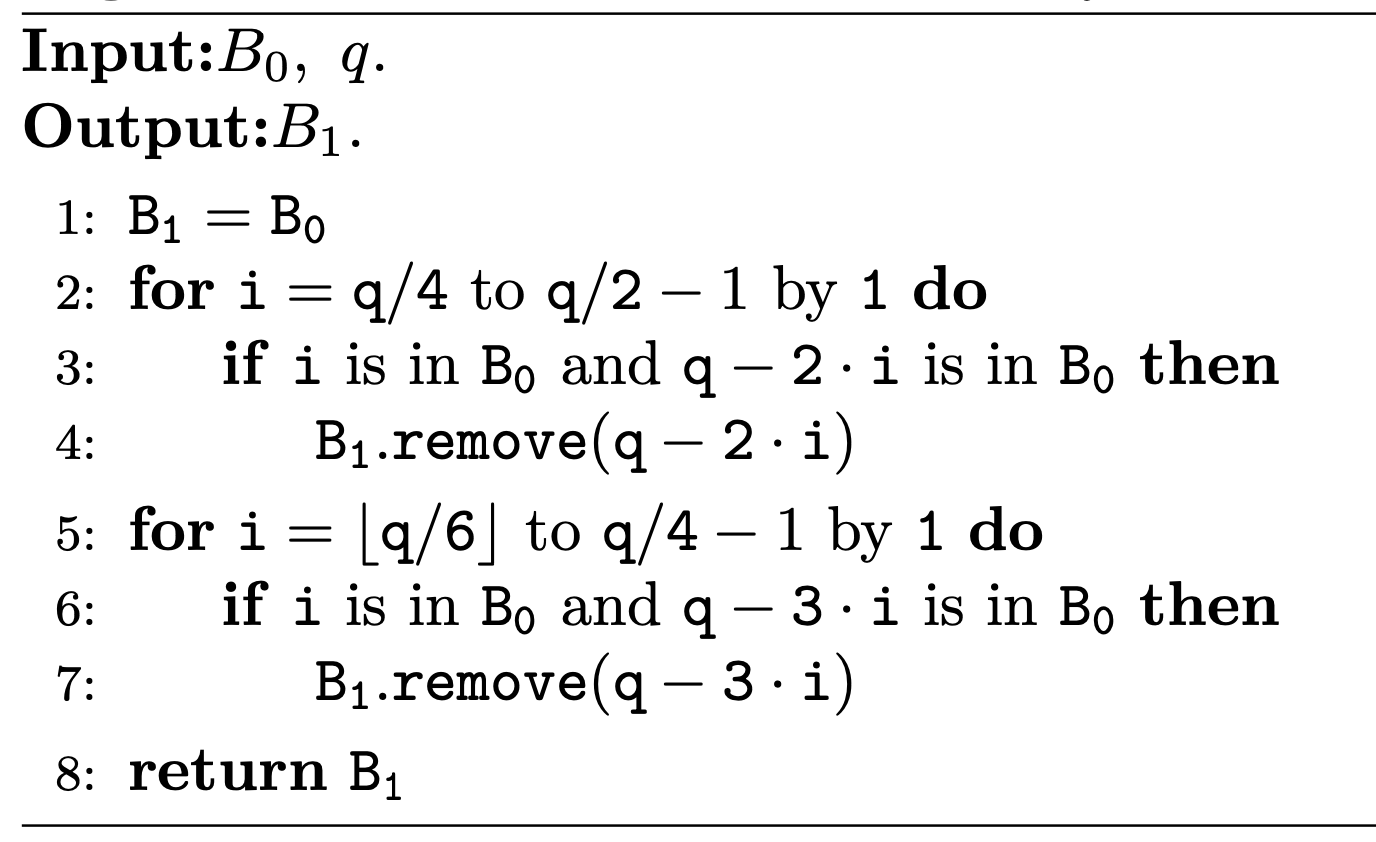
\includegraphics[width=0.63\linewidth]{Figures/alg_B1}
				\end{figure}
				\end{center}
%			{\footnotesize
%			\begin{algorithm}[H]
%			\caption{Construction of auxiliary set $B_1$} \label{alg_bucket_set_construction_B1}
%			\textbf{Input:}$B_0,\ q$.\\
%			\textbf{Output:}$B_1$.
%			\begin{algorithmic}[1]
%					\State $\mathtt{B_1 = B_0}$
%					\For{$\mathtt{i= q/4}$ to $\mathtt{q/2} -1$ by $\mathtt{1}$} 
%						\If {$\mathtt{i}$ is in $\mathtt{B_0}$ and $\mathtt{q -2\cdot i}$ is in $\mathtt{B_0}$}
%						\State $\mathtt{B_1.remove(q-2\cdot i)}$
%						\EndIf
%					\EndFor 
%					\For{$\mathtt{i= \lfloor q/6 \rfloor}$ to $\mathtt{q/4} -1$ by $\mathtt{1}$} 
%						\If {$\mathtt{i}$ is in $\mathtt{B_0}$ and $\mathtt{q -3\cdot i}$ is in $\mathtt{B_0}$}
%						\State $\mathtt{B_1.remove(q-3\cdot i)}$
%						\EndIf
%					\EndFor 
%					
%					\State \Return $\mathtt{B_1}$
%			\end{algorithmic}
%			\end{algorithm}
%			}
			\item<2-> The bucket set is constructed as $B = B_1 \cup B_2$.	
%			\item<3-> Note: Elements in the bucket set is no longer consecutive, a new accumulation algorithm is needed.		
		\end{itemize}

	\fillframe
\end{frame}

\begin{frame}
	\UWtitle{Comparison}
%	\vspace*{1cm}
$q = 2^c$ is the radix used to decompose the scalars, $h=\lceil{\log_qr}\rceil$. The time complexity of Pippenger's bucket set and Pippenger's variant hold if $ r \le q/2\cdot q^{h-1}$. The time complexity of our construction holds when $r/q^h$ is small.

\begin{table}[H]
\renewcommand*{\arraystretch}{1.1}
\centering
\caption{Comparison of different methods that computes $S_{n,r}$}
%\resizebox{\columnwidth}{!}{
\begin{tabularx}{\textwidth}{Rrr}
\toprule
{Method}   & {Storage} & { Complexity} \\ \midrule
Trivial method                   &     $n\cdot P$            &     ${3}/{2}\cdot (n\log_2{r})\cdot A$                        \\ 
%Binary addition chain               &    $2^c(n/c)\cdot P$             &      $2nh\cdot A  $             \\ \hline
Straus method     \cite{straus1964addition}                  &       $n 2^c\cdot P$          &        $h(n+c)\cdot A$       \\
Pippenger   \cite{pippenger1976evaluation,bernstein2012faster}      &      $n\cdot P$       &            $h(n+q/2)\cdot A$         \\ 
Pippenger variant \cite{brickell1995fast}  &    $ nh\cdot P$             &   $(nh+q/2)\cdot A$             \\

Our construction [this work]&    $ 3nh\cdot P$             &   $(nh+ 0.21 q)\cdot A$             \\ \bottomrule
\end{tabularx}%
%}
\label{table_methods_comparison}
\end{table}
%\fillframe
\end{frame}

\begin{frame}
	\UWtitle{Instantiation and experiment over BLS12-381 curve}
%	\vspace*{2cm}


\only<1>{
	\begin{figure}
		\centering
		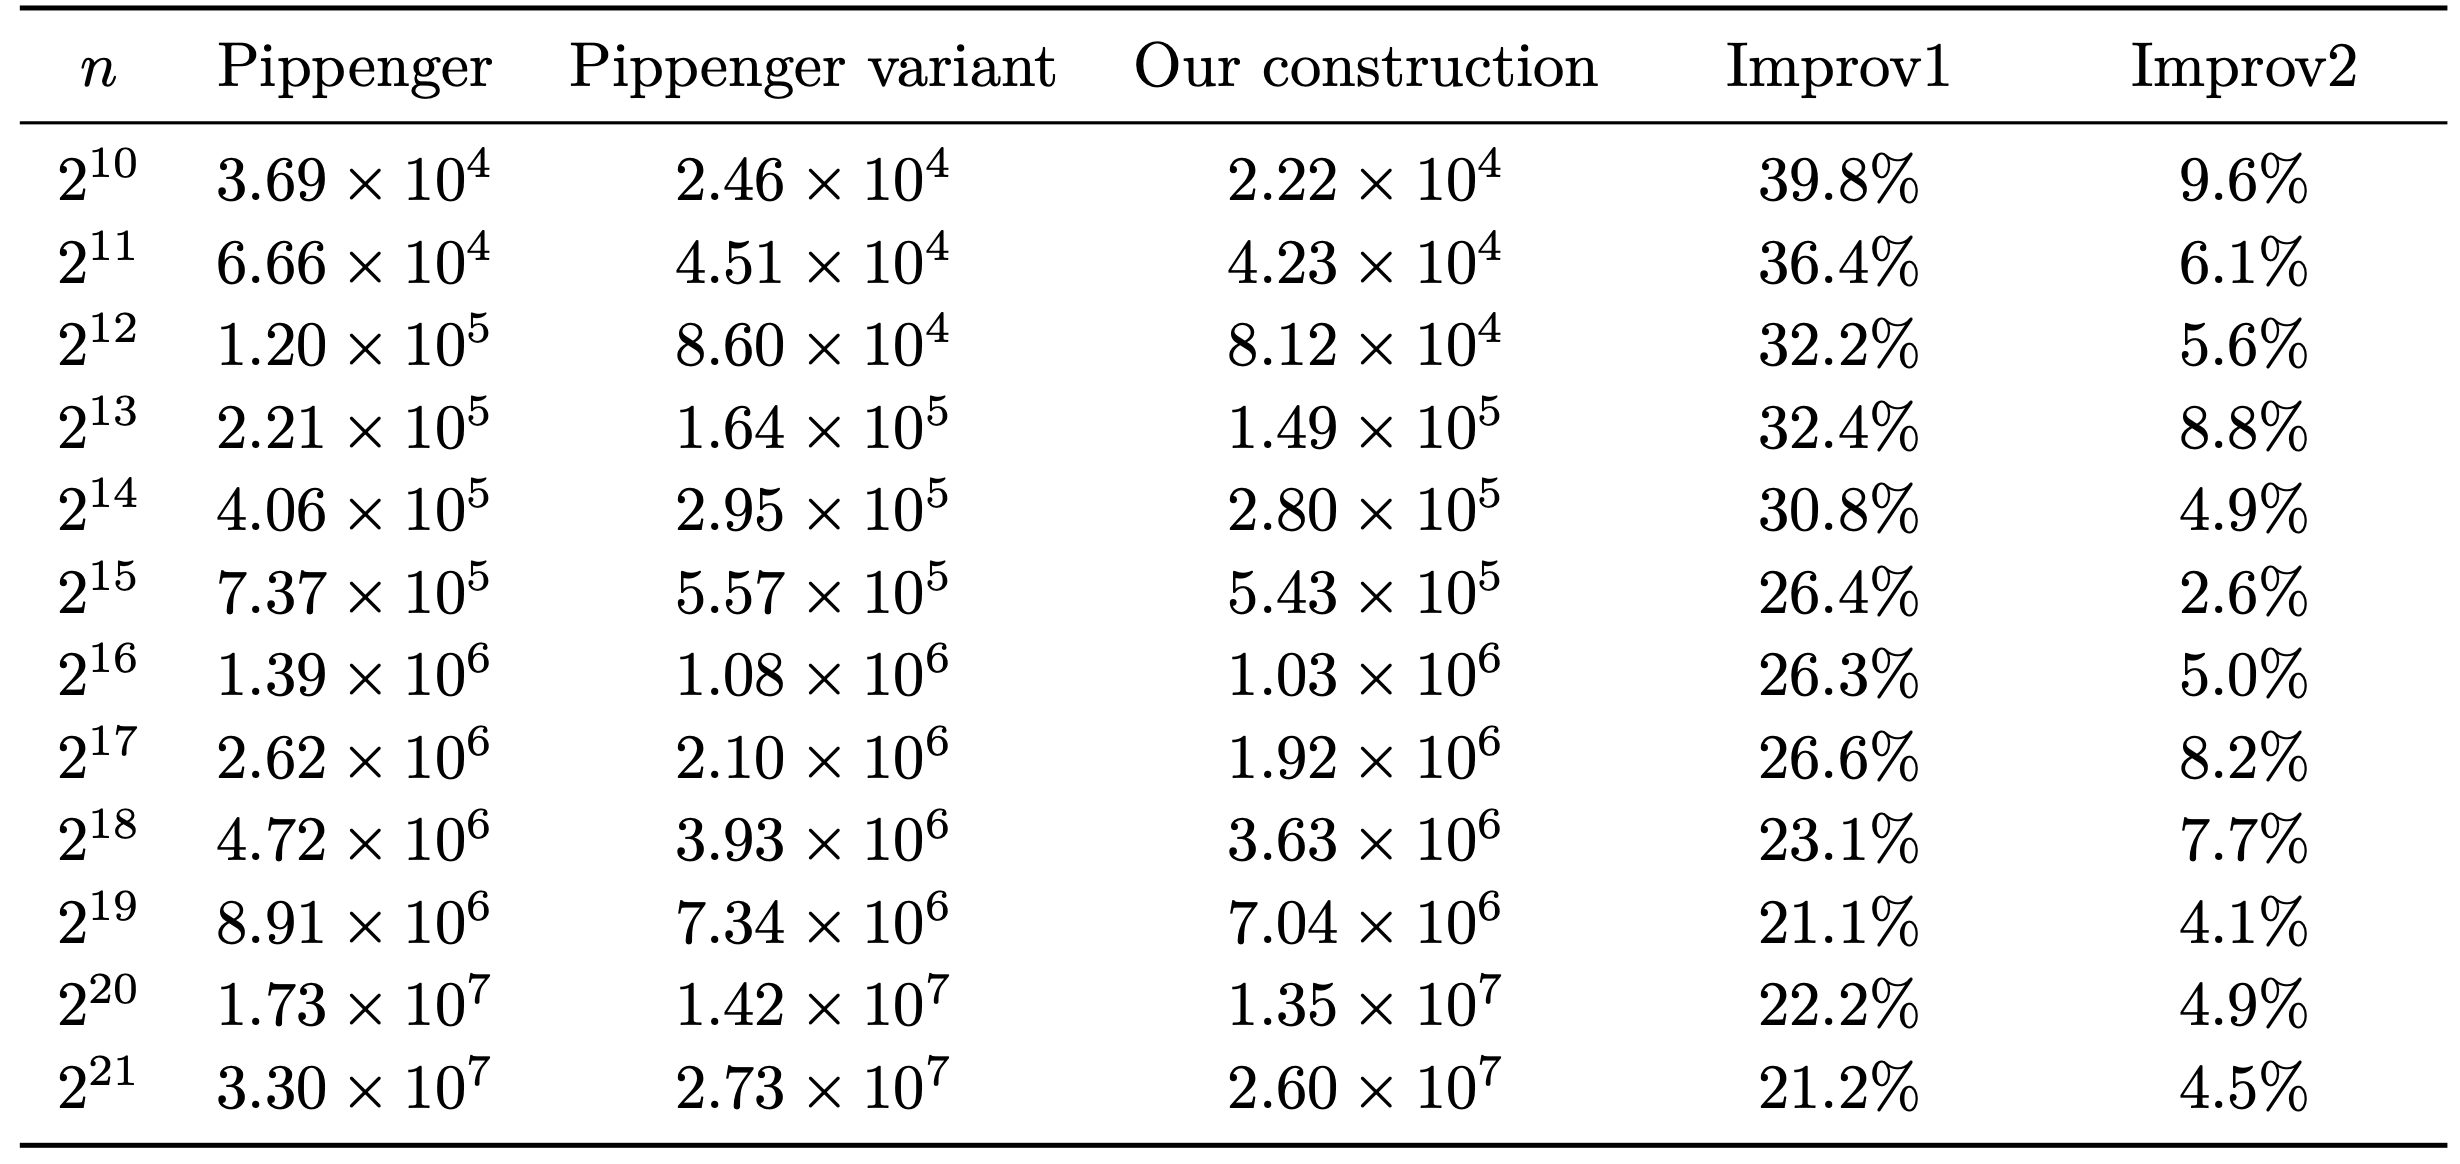
\includegraphics[width=\linewidth]{Figures/benchmark1}
	\end{figure}}
	
\only<2>{
		\begin{center}
		\begin{figure}
			\centering
			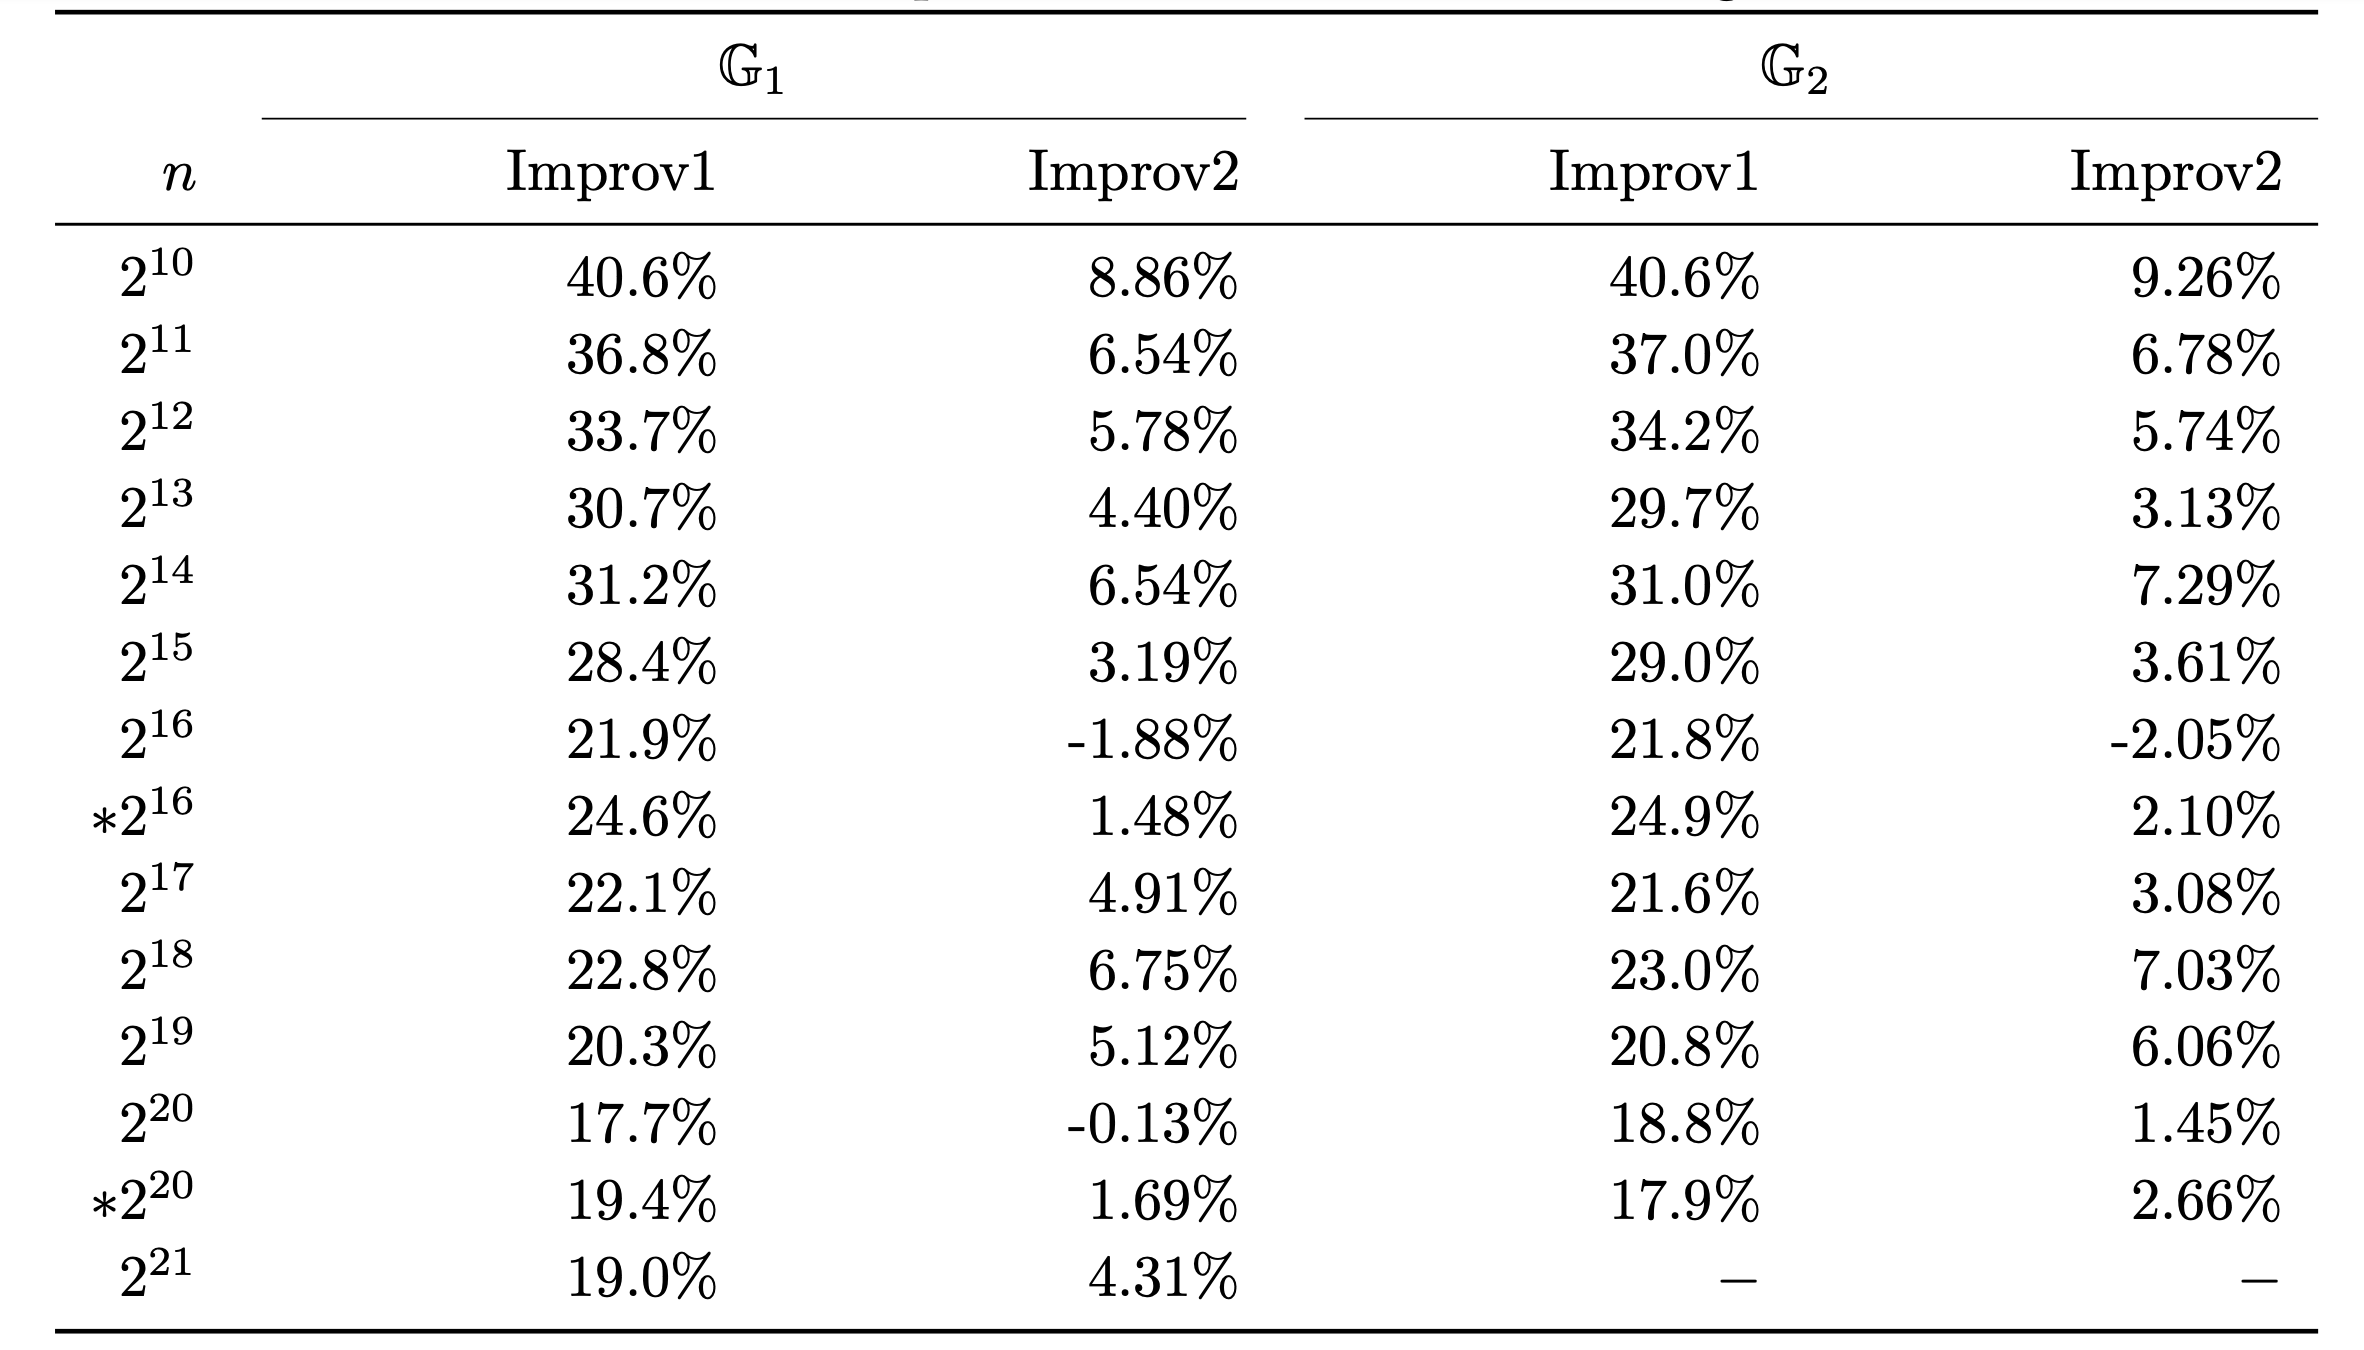
\includegraphics[width=\linewidth]{Figures/benchmark2}
		\end{figure}
		\end{center}
		}

%	\fillframe
\end{frame}


\begin{frame}
%	\UWtitle{Conclusion}
%	\vspace*{1cm}
	
	    \begin{block}{Conclusions:}
	        \begin{itemize}
	           \item 	$S_{n,r}$ over fixed points can be computed using at most $$\approx nh + 0.21q$$
	           								additions, with the help of $3 nh$ precomputed points
	           								\begin{equation*}
	           								\left\{mq^jP_i\ |\ 1\le i\le n,0\le j\le  h -1,m\in \{1,2,3\}\right\},
	           								\end{equation*}	
	           			where $q=2^c$ is selected to minimize the complexity, $h = \lceil \log_q r\rceil$, $r/q^h$ is small.
	           \vspace{0.1in}
	           
	           \item Over BLS12-381 curve, when computing $n$-scalar multiplications for $n = 2^{e}\ (10\le e \le 21)$.
	                \begin{itemize}
	                \item[-] $21\%+$ improvement against Pippenger's bucket method.
	                \item[-] $2.6\%$ to $9.6\%$ improvement against the variant \cite{brickell1995fast}.
	                \end{itemize}
	        \end{itemize}
	        \end{block}
		
%	\fillframe
\end{frame}



\begin{frame}<beamer:0> %  Hide the references

\vspace{0.75in}
%	\vspace*{1.5cm}
\bibliographystyle{alpha}
\bibliography{../references-for-all-guiwen.bib}
%\fillframe
\end{frame}



%\input{MSM-RIPPLE.tex}

\end{document}
